\section*{Analysis}
\label{sec:analysis}

The emulator is used to perform the debugging (although it does not seem to be able to run RenderScript code).
To run the code, we are using two devices for the analysis.
The first is a Nexus 7 with the following specs:

\begin{verbatim}
    CPU: Qualcomm Snapdragon S4 Pro, 1.5GHz
    GPU: Adreno 320, 400MHz
    Memory - 2 GB
    Storage 32 GB
\end{verbatim}

The second is a Samsung Galaxy Nexus with the following specs:

\begin{verbatim}
    CPU: ARMv7, 2 cores, 1200 Mhz, SIMD NEON
    Memory: 694, JVM max: 96 MB
    GPU: PowerVR SGX 540.
\end{verbatim}


\subsection*{Perliminary Results}

While we do have implementations for 3 out of the 4 benchmarks we promised in the proposal schedule,
  our results only show part of those.
The data has not been fully analyzed, but we can give some perliminary insights into the expected
  results.


\begin{figure}[t!]
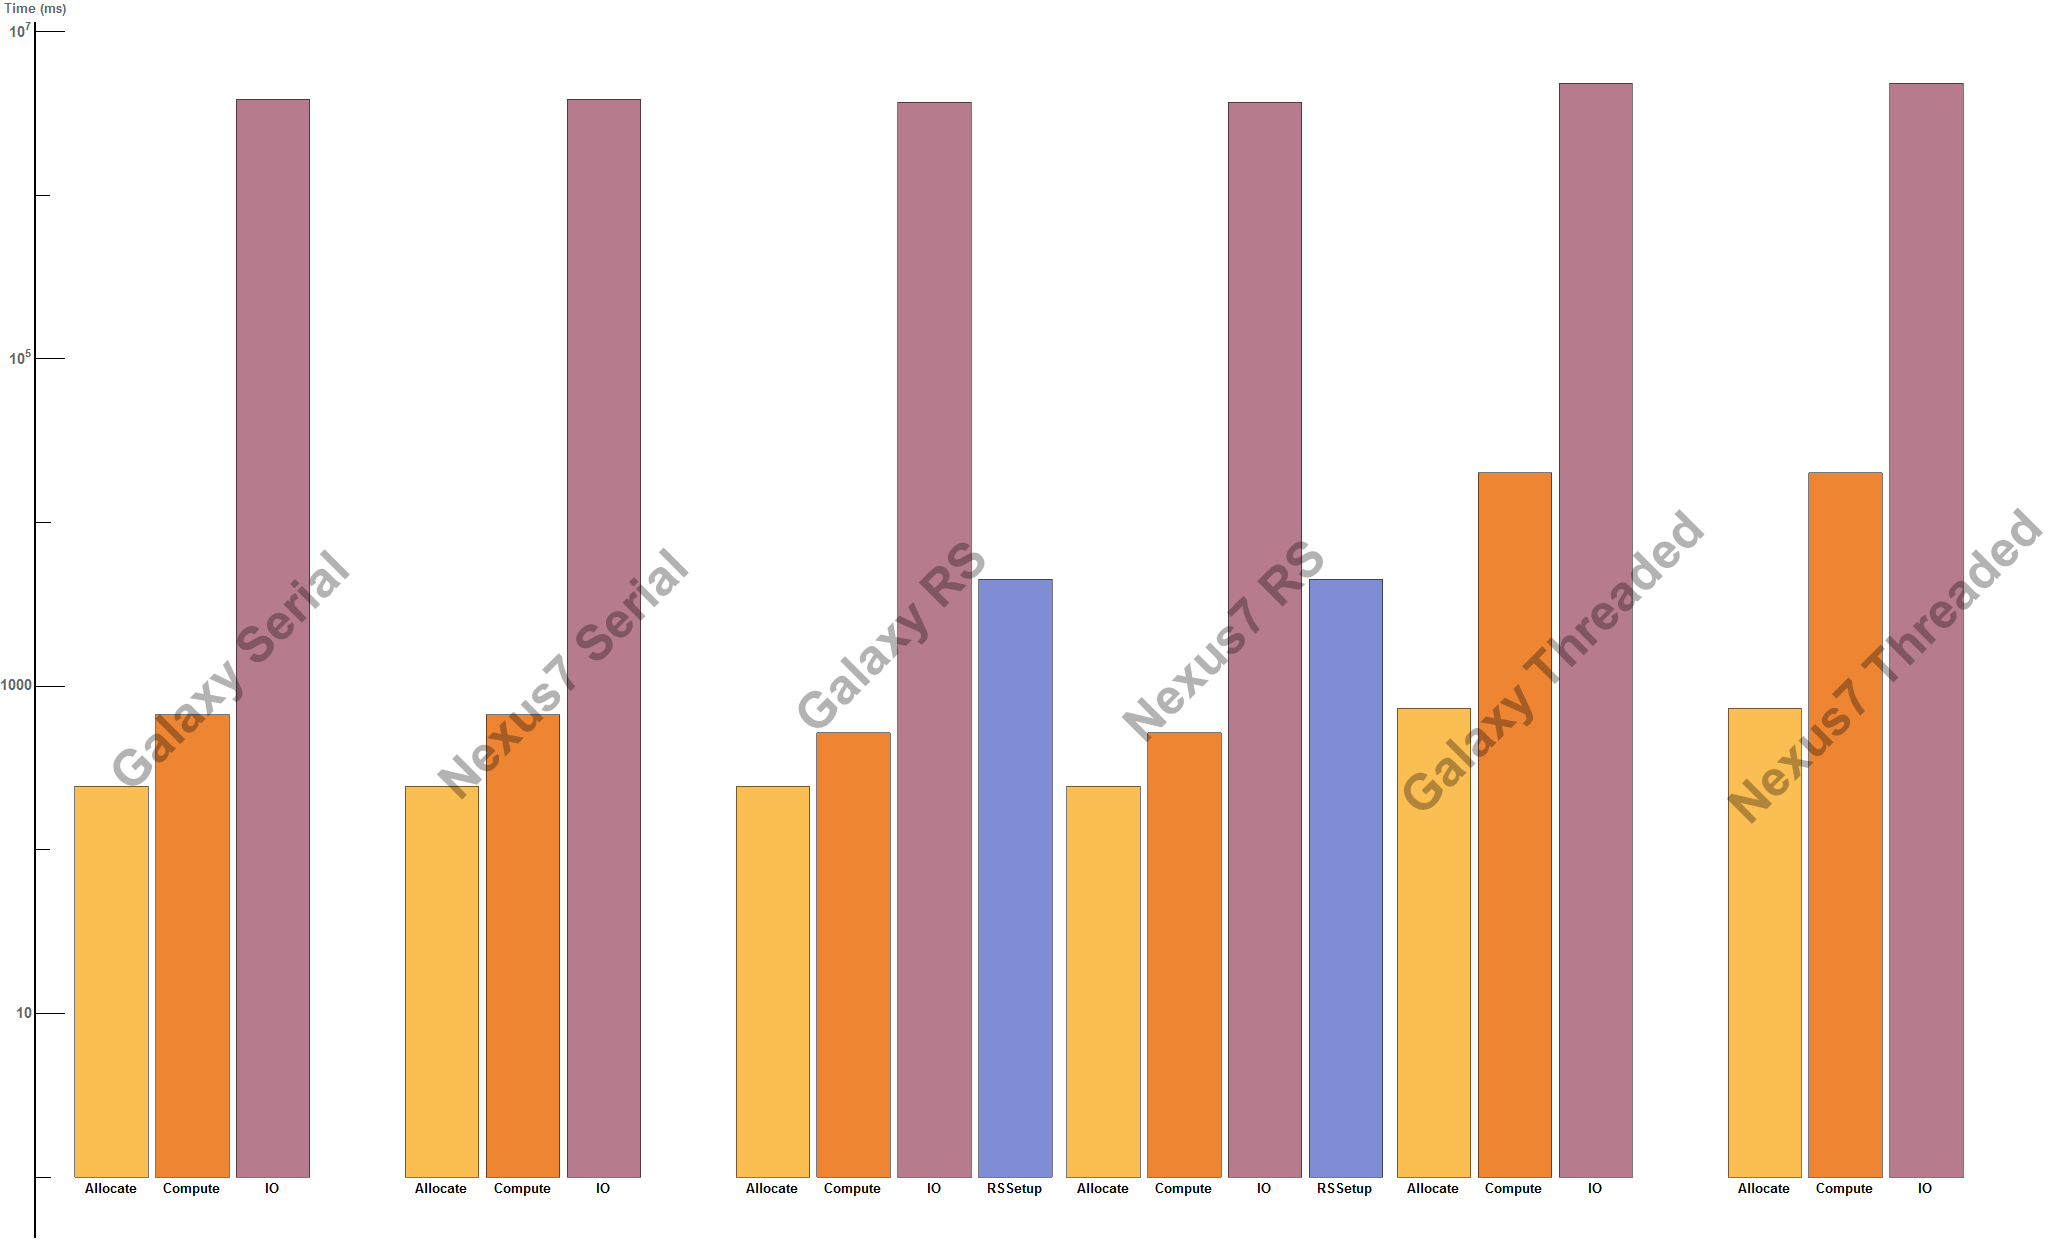
\includegraphics[scale=0.125]{VectorAdd.png}
\caption{VectorAdd Benchmark.}
\label{fig:vecadd}
\centering
\end{figure}



\begin{figure}[t!]
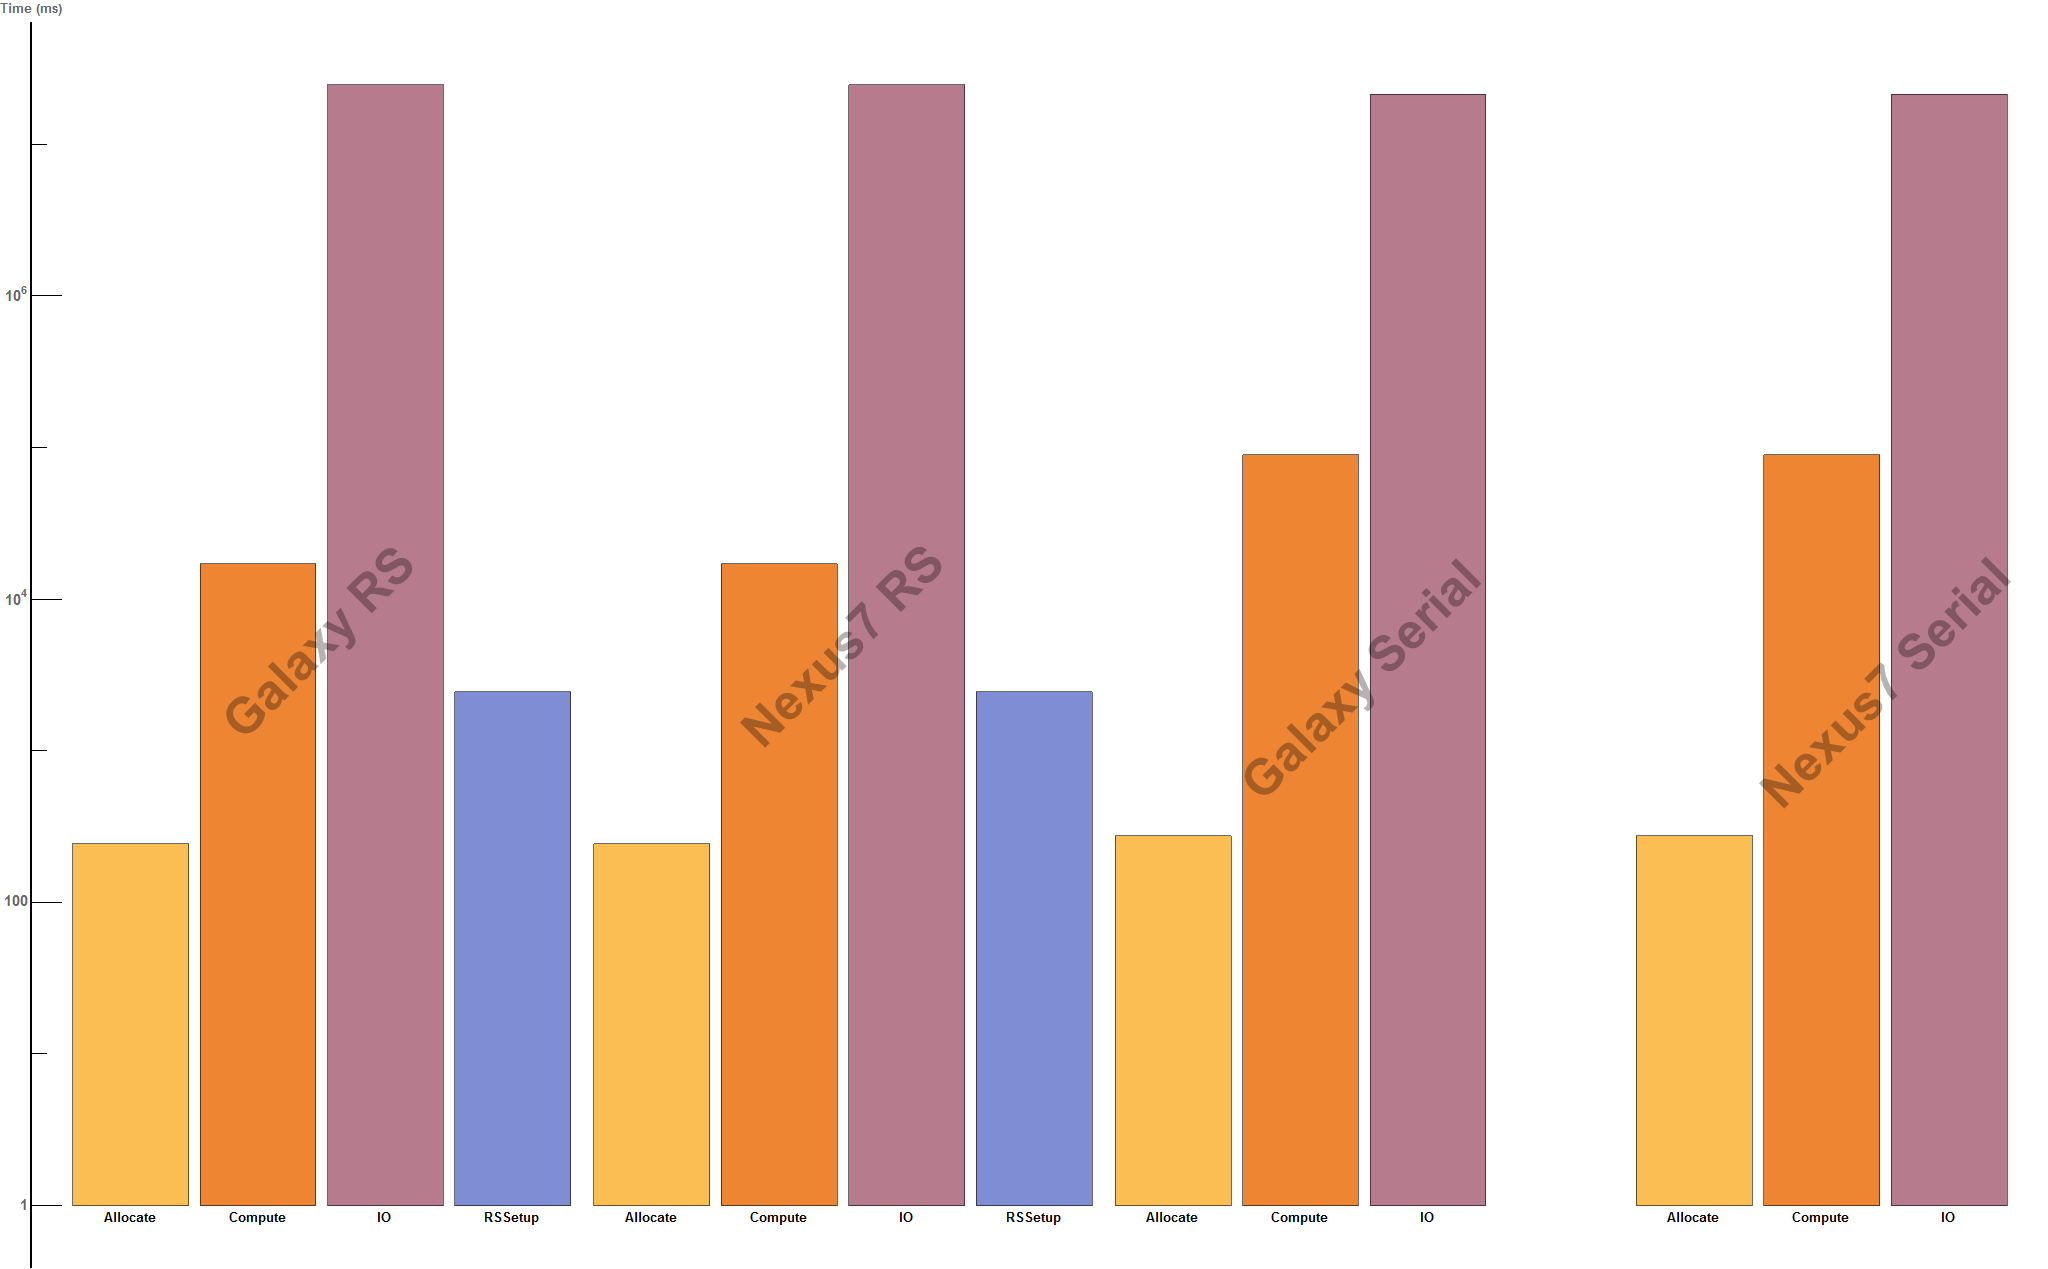
\includegraphics[scale=0.125]{Sgemm.png}
\caption{Matrix Matrix Multiplication Benchmark.}
\label{fig:sgemm}
\centering
\end{figure}



In figure~\ref{fig:stencil}, we should the results from running the stencil code across the different
  implementations.

The serial versions have an added {\tt RSSetup} time, this is either due to bad parsing of the 
  output data or an incorrect labeling of a timer in the source code.

\begin{figure}[t!]
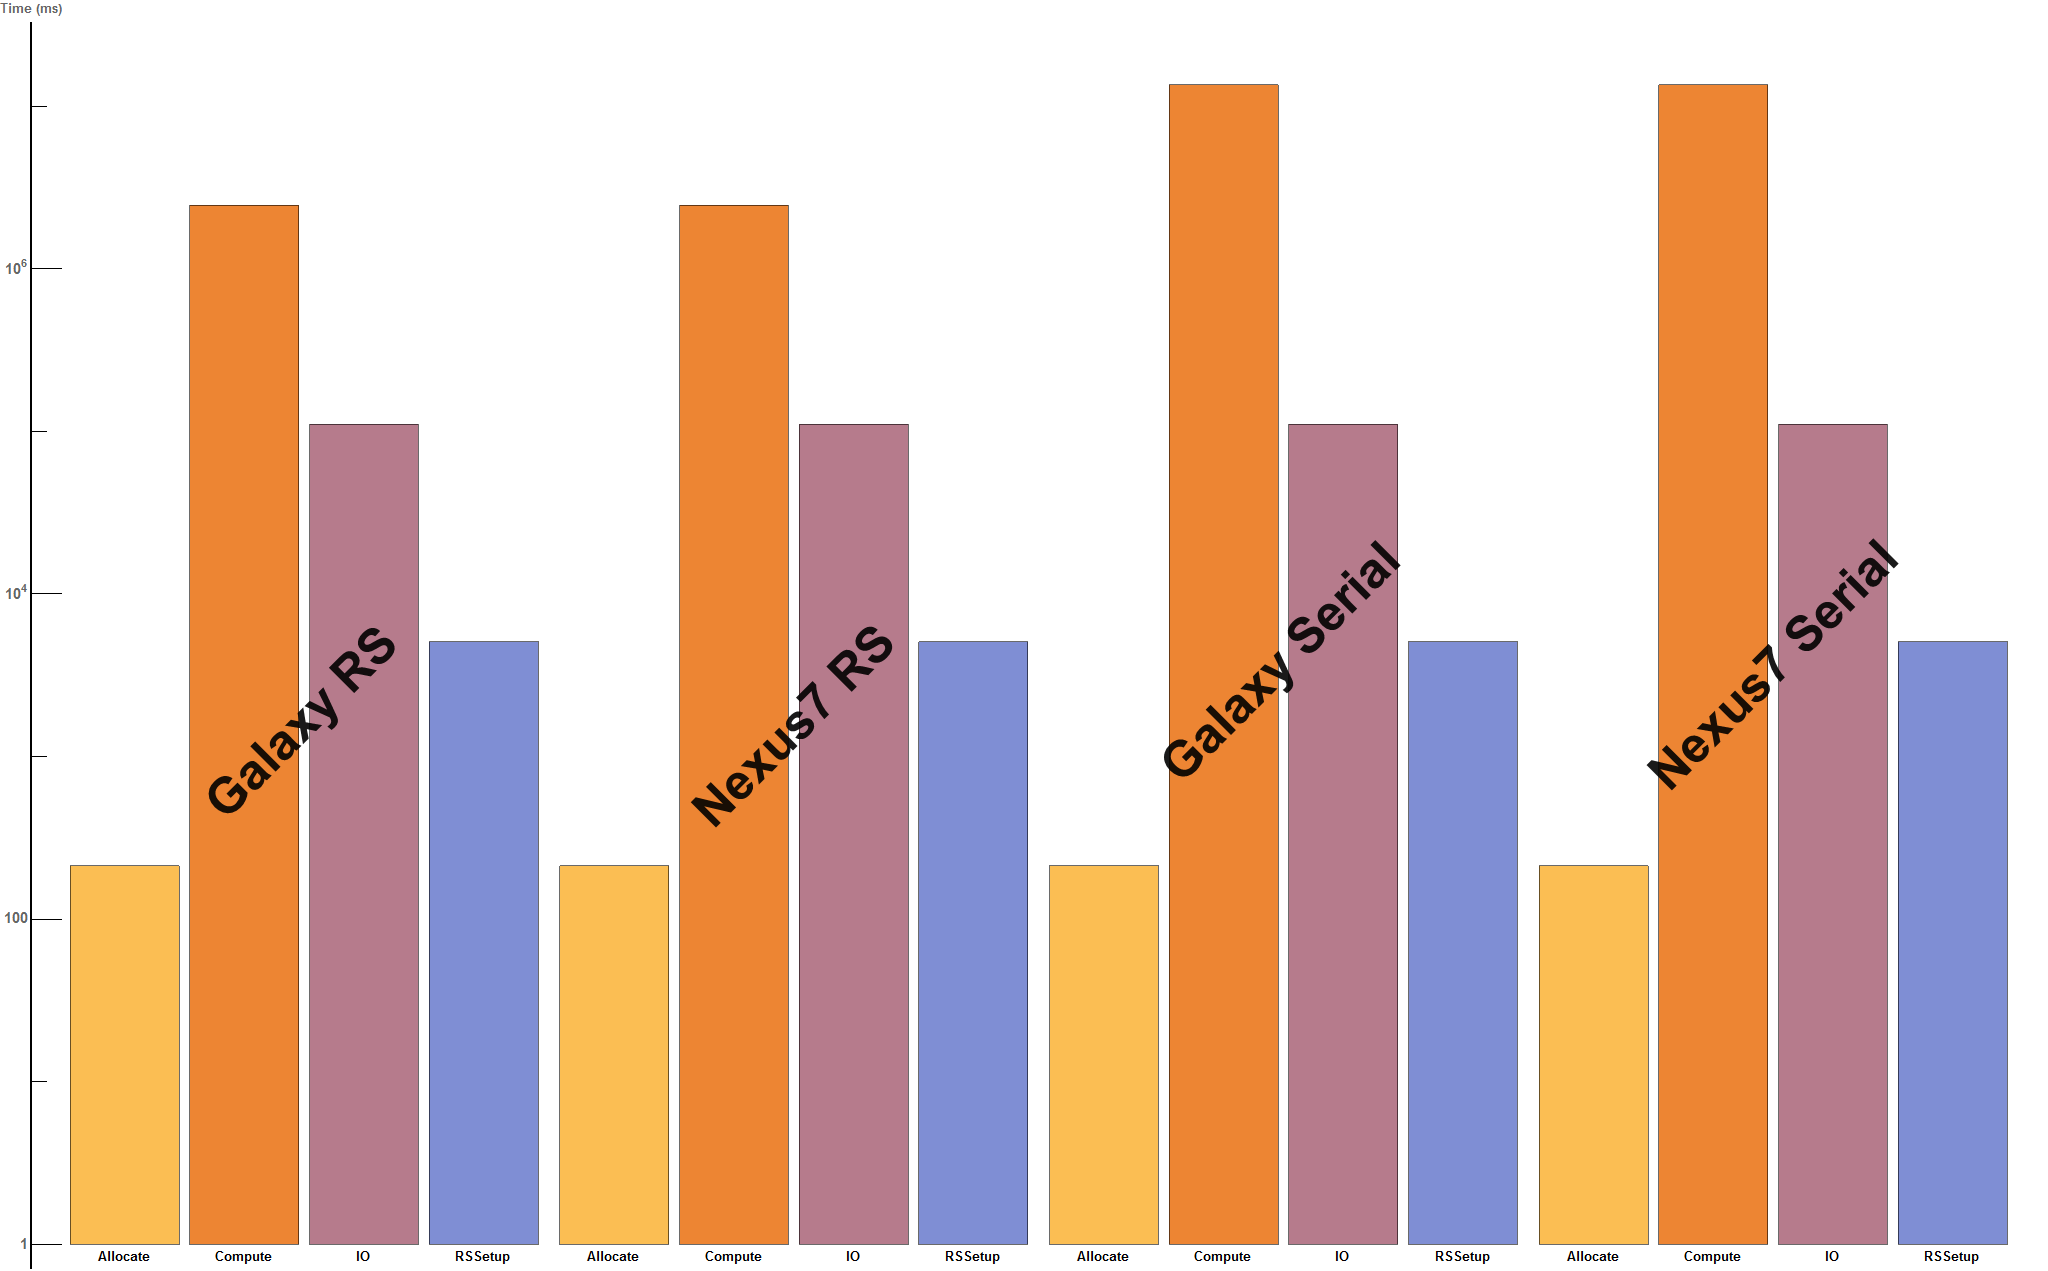
\includegraphics[scale=0.125]{Stencil.png}
\caption{Stencil Benchmark.}
\label{fig:stencil}
\centering
\end{figure}


While these graphs have the infromation, they are not presented in the clearest way.
Future work would remove the IO times from the plots, this would avoid us having to use Log scalling
  and would make some of the differences more visable.
  

